\documentclass[aspectratio=169]{beamer}
\usetheme{Metropolis}
\setbeamertemplate{blocks}[default]

\usepackage[utf8]{inputenc}
\usepackage[spanish,es-tabla]{babel}
\usepackage{lmodern}
\usepackage{amsmath,amssymb}
\usepackage{booktabs}
\usepackage{array}
\usepackage{graphicx}
\usepackage{tikz}
\usetikzlibrary{arrows.meta,positioning,fit,backgrounds,shapes.geometric}
\usepackage{xcolor}
\usepackage{colortbl}
\usepackage{listings}

\definecolor{entra}{HTML}{2E7D32}
\definecolor{sale}{HTML}{8C1D40}
\definecolor{pivcolor}{HTML}{D2691E}
\definecolor{basecolor}{HTML}{3B7EA1}

\lstset{
  basicstyle=\ttfamily\scriptsize,
  breaklines=true,
  columns=fullflexible,
  keywordstyle=\color{basecolor}\bfseries,
  commentstyle=\color{gray},
  stringstyle=\color{entra}
}

\title{Programación Lineal: el método Simplex, paso a paso}
\subtitle{De las ecuaciones a los tableaux --- y los casos degenerados}
\author{Métodos de Optimización --- Maestría}
\institute{Universidad Pontificia Bolivariana}
\date{}

\begin{document}

\maketitle

% ================= SECCION 1 =================
\section{Motivación y forma estándar}

\begin{frame}{¿Dónde estamos?}
En las Clases 1--3 optimizamos funciones \emph{sin restricciones lineales explícitas} (gradiente, Hessiana, Lagrange, KKT) y luego exploramos búsquedas \emph{numéricas} (bisección, áurea, metaheurísticas).

\vspace{0.4cm}
Hoy cambiamos de terreno: \textbf{programación lineal (PL)} --- función objetivo lineal, restricciones lineales.
\par\medskip
\begin{block}{La buena noticia}
Para PL existe un método \emph{exacto}, finito y muy estructurado: el \textbf{Simplex} (Dantzig, 1947). No aproxima: encuentra el óptimo exacto en un número finito de pasos.
\end{block}
\par\medskip
\begin{alertblock}{El objetivo de hoy}
Antes de usar el tableau simplex ``de memoria'', vamos a construirlo \emph{nosotros mismos}: sistema de ecuaciones $\to$ elegir variables base $\to$ diagonalizar a mano $\to$ iterar. El tableau aparecerá al final como una forma compacta de anotar exactamente lo mismo.
\end{alertblock}
\end{frame}

\begin{frame}{Forma estándar de un problema de PL}
Un problema de PL en \textbf{forma estándar}:
\[
\begin{aligned}
\max \quad & z = c_1 x_1 + c_2 x_2 + \dots + c_n x_n \\
\text{s.a.} \quad & a_{i1}x_1 + a_{i2}x_2 + \dots + a_{in}x_n = b_i, \quad i=1,\dots,m \\
& x_1,\dots,x_n \geq 0
\end{aligned}
\]

\begin{itemize}
\item Objetivo lineal, restricciones lineales, variables no negativas.
\item Restricciones en \textbf{igualdad} (no $\leq$ o $\geq$).
\item $b_i \geq 0$ (se puede lograr multiplicando por $-1$ si hace falta).
\end{itemize}
\par\medskip
\begin{block}{¿Y si mi problema no viene así?}
$\leq$ se convierte en $=$ sumando una \textbf{variable de holgura} (\emph{slack}); $\geq$ restando una variable de \textbf{exceso}; una restricción de igualdad ``fea'' o una variable libre requieren trucos adicionales (Clase futura: método de dos fases / Big M).
\end{block}
\end{frame}

\begin{frame}{Variables de holgura: de $\leq$ a $=$}
Si la restricción original es
\[
a_{i1}x_1 + \dots + a_{in}x_n \leq b_i,
\]
se introduce una variable de holgura $s_i \geq 0$ que ``absorbe'' la diferencia:
\[
a_{i1}x_1 + \dots + a_{in}x_n + s_i = b_i.
\]
\par\medskip
\begin{exampleblock}{Interpretación física}
$s_i$ es literalmente \emph{cuánto recurso sobra} si no se usa toda la restricción $i$. $s_i=0$ significa que la restricción se cumple con igualdad (está ``activa'' / ``ajustada'').
\end{exampleblock}

Cada restricción $\leq$ aporta \textbf{una} variable de holgura nueva, con coeficiente $+1$ solo en su propia ecuación (coeficiente $0$ en las demás) --- esto será clave en un momento.
\end{frame}

% ================= SECCION 2 =================
\section{El ejemplo que resolveremos a mano}

\begin{frame}{Nuestro problema guía}
\begin{block}{Problema (Wyndor Glass Co. --- clásico de Hillier \& Lieberman)}
Una fábrica produce dos productos, con ganancia $3$ y $5$ (miles de \$) por unidad. Tres líneas de producción limitan la capacidad:
\[
\begin{aligned}
\max \quad & z = 3x_1 + 5x_2 \\
\text{s.a.} \quad & x_1 \leq 4 \\
& 2x_2 \leq 12 \\
& 3x_1 + 2x_2 \leq 18 \\
& x_1, x_2 \geq 0
\end{aligned}
\]
\end{block}
Solo 2 variables: podemos \textbf{dibujarlo} y verificar geométricamente cada paso que demos algebraicamente.
\end{frame}

\begin{frame}{Paso 1: forma estándar con holguras}
Añadimos $s_1,s_2,s_3\geq0$, una por restricción:
\[
\begin{aligned}
x_1 + s_1 &= 4 \\
2x_2 + s_2 &= 12 \\
3x_1 + 2x_2 + s_3 &= 18
\end{aligned}
\]
con $z - 3x_1 - 5x_2 = 0$ (escribimos el objetivo también como una ecuación, moviendo todo a la izquierda).

\vspace{0.3cm}
\textbf{5 incógnitas ($x_1,x_2,s_1,s_2,s_3$), 3 ecuaciones.} Un sistema así tiene infinitas soluciones (2 grados de libertad) --- necesitamos un criterio para elegir \emph{cuáles} resolver.
\end{frame}

\begin{frame}{Paso 2: variables básicas y no básicas}
\begin{block}{La idea central del Simplex}
De las $n$ variables, elegimos $m$ para que sean \textbf{básicas} (se resuelven en función de las demás) y las $n-m$ restantes las fijamos en \textbf{cero}: son \textbf{no básicas}.
\end{block}

Con $m=3$ ecuaciones y $n=5$ variables, elegimos 3 variables básicas. Cada elección posible (si es factible, es decir, valores $\geq 0$) es un \textbf{vértice} de la región factible.

\vspace{0.3cm}
\textbf{¿Por qué vértices?} Es un resultado geométrico clave de PL: si el óptimo existe, siempre hay un vértice óptimo. El Simplex recorre vértices adyacentes mejorando $z$ en cada paso, en vez de revisar el interior de la región (que es infinito).
\end{frame}

\begin{frame}{Paso 3: la base inicial ``regalada''}
¿Con qué base empezamos? Con las variables de holgura: $\{s_1,s_2,s_3\}$.
\par\medskip
\begin{block}{¿Por qué son la elección natural?}
Cada $s_i$ aparece con coeficiente $+1$ en \emph{su propia} ecuación y $0$ en las demás --- el sistema \textbf{ya está diagonalizado} respecto a esa base, sin necesidad de hacer ninguna eliminación:
\[
\begin{pmatrix}1&0&0\\0&1&0\\0&0&1\end{pmatrix}
\begin{pmatrix}s_1\\s_2\\s_3\end{pmatrix}
=
\begin{pmatrix}4\\12\\18\end{pmatrix}
\quad\text{con } x_1=x_2=0.
\]
\end{block}
Solución básica factible (SBF) inicial: $x_1=0,\ x_2=0,\ s_1=4,\ s_2=12,\ s_3=18$, y $z=0$. Geométricamente: el origen, siempre un vértice factible cuando todas las restricciones son $\leq$ con $b_i\geq0$.
\end{frame}

\begin{frame}{Región factible y lo que viene}
\centering
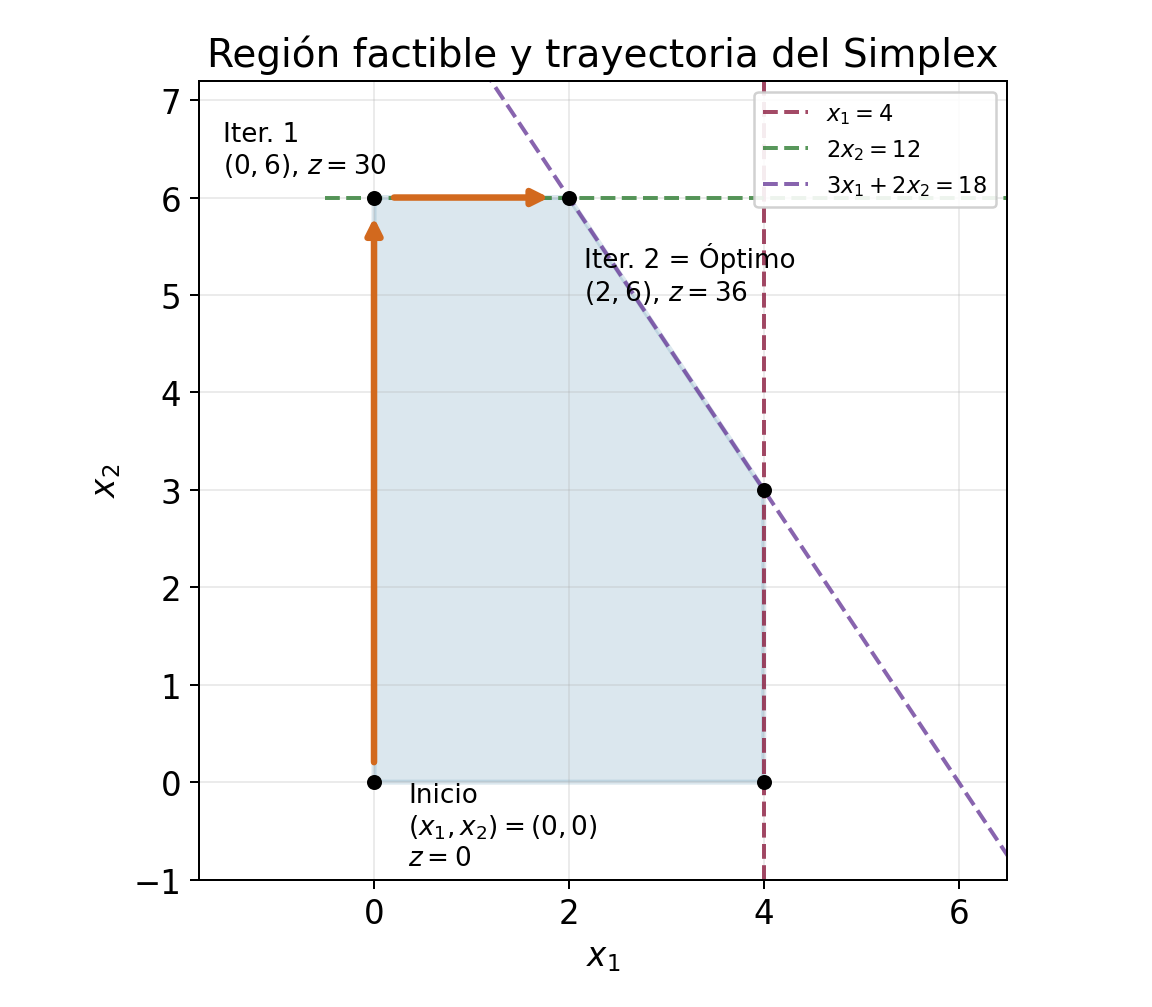
\includegraphics[width=0.62\textwidth]{figs/fig01_region_factible.png}

{\footnotesize Vamos a recorrer, a mano, los vértices marcados con flechas: $(0,0)\to(0,6)\to(2,6)$.}
\end{frame}

% ================= SECCION 3 =================
\section{Iteración 1: a mano, ecuación por ecuación}

\begin{frame}{¿Cómo saber si ya somos óptimos?}
Escribimos $z$ \textbf{en función de las variables no básicas} (aquí, $x_1,x_2$, porque las básicas $s_1,s_2,s_3$ ya están despejadas):
\[
z = 3x_1 + 5x_2.
\]
\par\medskip
\begin{block}{Criterio de optimalidad (problema de maximización)}
Si \emph{todo} coeficiente de las variables no básicas en la fila de $z$ es $\leq 0$, ninguna variable no básica puede seguir aumentando $z$: \textbf{ya somos óptimos}. Si algún coeficiente es positivo, esa variable, al crecer desde 0, todavía mejora $z$.
\end{block}

Aquí $3>0$ y $5>0$: \textbf{no somos óptimos}. Elegimos la variable con mayor coeficiente positivo para \textbf{entrar} a la base: $x_2$ (coeficiente $5$).
\end{frame}

\begin{frame}{¿Hasta dónde puede crecer $x_2$?}
Dejamos $x_1=0$ fijo y aumentamos $x_2$ desde 0. Cada ecuación nos dice cuánto puede crecer $x_2$ antes de que \emph{alguna} variable básica se vuelva negativa (lo cual violaría factibilidad):
\[
\begin{aligned}
s_1 &= 4 - x_1 = 4 &&\text{(no involucra a $x_2$: sin límite por esta fila)}\\
s_2 &= 12 - 2x_2 \geq 0 &\Rightarrow& \quad x_2 \leq 12/2 = 6\\
s_3 &= 18 - 2x_2 \geq 0 &\Rightarrow& \quad x_2 \leq 18/2 = 9
\end{aligned}
\]
\par\medskip
\begin{alertblock}{Regla de la razón mínima (\emph{minimum ratio test})}
El límite real es el \textbf{más restrictivo}: $x_2 \leq \min(6,9) = 6$. La fila que impone ese límite ($s_2$) es la que se queda en \textbf{cero} primero $\to$ esa variable \textbf{sale} de la base.
\end{alertblock}

Entra $x_2$, sale $s_2$.
\end{frame}

\begin{frame}{Paso clave: diagonalizar a mano respecto a la nueva base}
Queremos que el sistema vuelva a estar ``diagonalizado'', ahora para la base $\{s_1, x_2, s_3\}$. Partimos de
\[
\begin{aligned}
x_1 \phantom{{}+{}2x_2} &\hphantom{{}={}}+ s_1 &&= 4 \\
2x_2 \hphantom{{}+{}x_1} &\hphantom{{}={}} + s_2 &&= 12 \\
3x_1 + 2x_2 \hphantom{{}+{}s_1} &\hphantom{{}={}} + s_3 &&= 18
\end{aligned}
\]

\textbf{(a) Normalizar la fila pivote} (dividir por el coeficiente de $x_2$, que es $2$):
\[
x_2 + \tfrac{1}{2}s_2 = 6 \qquad \text{\small (fila de $s_2$ dividida entre 2)}
\]
\end{frame}

\begin{frame}{Eliminación de Gauss-Jordan, fila por fila}
\textbf{(b) Eliminar $x_2$ de las demás filas} restando el múltiplo adecuado de la fila pivote:

\begin{itemize}
\item Fila de $s_1$: no contiene $x_2$ (coeficiente 0) $\to$ \textbf{no cambia}: $\ x_1 + s_1 = 4$.
\item Fila de $s_3$: coeficiente de $x_2$ es $2$, igual que en la fila pivote ya normalizada $\times 2$. Restamos $2\times(x_2+\tfrac12 s_2=6)$ de $(3x_1+2x_2+s_3=18)$:
\[
3x_1 + 2x_2 + s_3 - 2\left(x_2+\tfrac12 s_2\right) = 18 - 2(6)
\ \Longrightarrow\
3x_1 - s_2 + s_3 = 6.
\]
\item Fila de $z$: $z-3x_1-5x_2=0$. Sumamos $5\times(x_2+\tfrac12 s_2=6)$ para eliminar $x_2$:
\[
z - 3x_1 - 5x_2 + 5\left(x_2+\tfrac12 s_2\right) = 0+5(6)
\ \Longrightarrow\
z - 3x_1 + \tfrac{5}{2}s_2 = 30.
\]
\end{itemize}
\end{frame}

\begin{frame}{Sistema tras la iteración 1 --- ya diagonalizado}
\[
\begin{aligned}
x_1 &&&+\, s_1 &&&&= 4\\
&& x_2 &&+\,\tfrac12 s_2 &&&= 6\\
3x_1 &&& &&-\,s_2\,+\,s_3 &&= 6\\
\hline
z &-3x_1 & & &+\,\tfrac52 s_2 & && = 30
\end{aligned}
\]

Nueva SBF: $x_1=0,\ x_2=6,\ s_1=4,\ s_2=0,\ s_3=6,\ z=30$. Verifica contra la figura: es exactamente el vértice $(0,6)$.
\par\medskip
\begin{block}{¿Ya terminamos?}
$z = 30 + 3x_1 - \tfrac52 s_2$. El coeficiente de $x_1$ es $+3>0$: \textbf{todavía se puede mejorar} aumentando $x_1$. Seguimos iterando.
\end{block}
\end{frame}

% ================= SECCION 4 =================
\section{Iteración 2 y verificación de optimalidad}

\begin{frame}{Iteración 2: entra $x_1$}
Fila de $z$: $z = 30 + 3x_1 - \tfrac52 s_2$. Único coeficiente positivo: $x_1$ (coeficiente $3$) $\to$ \textbf{entra $x_1$}.

Razón mínima (con $x_2$ fijo en su fila, $s_2=0$ no básico):
\[
\begin{aligned}
s_1: \quad x_1 + s_1 = 4 &\ \Rightarrow\ x_1 \leq 4/1 = 4\\
x_2: \quad \text{coeficiente de $x_1$ es } 0 &\ \Rightarrow\ \text{sin límite por esta fila}\\
s_3: \quad 3x_1 + s_3 = 6\ (\text{con } s_2{=}0) &\ \Rightarrow\ x_1 \leq 6/3 = 2
\end{aligned}
\]

Mínimo: $2$, en la fila de $s_3$ $\to$ \textbf{sale $s_3$}.
\end{frame}

\begin{frame}{Diagonalizar otra vez}
Fila pivote ($s_3$), normalizada (dividir entre $3$):
\[
x_1 - \tfrac13 s_2 + \tfrac13 s_3 = 2
\]

Eliminar $x_1$ de las demás filas:
\[
\begin{aligned}
s_1:\ & (x_1+s_1=4) - 1\times(x_1-\tfrac13 s_2+\tfrac13 s_3=2) \ \Rightarrow\ s_1 + \tfrac13 s_2 - \tfrac13 s_3 = 2\\[2pt]
x_2:\ & \text{coeficiente de $x_1$ ya era 0} \ \Rightarrow\ \text{no cambia: } x_2 + \tfrac12 s_2 = 6\\[2pt]
z:\ & (z-3x_1+\tfrac52 s_2=30) + 3\times(x_1-\tfrac13 s_2+\tfrac13 s_3=2) \ \Rightarrow\ z + \tfrac32 s_2 + s_3 = 36
\end{aligned}
\]
\end{frame}

\begin{frame}{Sistema final --- ¿es óptimo?}
\[
\begin{aligned}
&&&s_1 &+\,\tfrac13 s_2 &-\,\tfrac13 s_3 &&= 2\\
&x_2 & & &+\,\tfrac12 s_2 & &&= 6\\
x_1& & & &-\,\tfrac13 s_2 &+\,\tfrac13 s_3&&= 2\\
\hline
z& & & &+\,\tfrac32 s_2 &+\,s_3 && = 36
\end{aligned}
\]
\par\medskip
\begin{alertblock}{Criterio de optimalidad --- se cumple}
$z = 36 - \tfrac32 s_2 - s_3$: \textbf{todo} coeficiente de las no básicas ($s_2,s_3$) en la fila de $z$ es $\leq 0$. Ningún intercambio mejora $z$: \textbf{óptimo alcanzado}.
\end{alertblock}

\textbf{Solución óptima:} $x_1^\ast=2,\ x_2^\ast=6,\ z^\ast=36$ --- exactamente el vértice marcado en la figura anterior.
\end{frame}

\begin{frame}{Repaso del camino completo}
\begin{center}
\begin{tabular}{@{}lccc@{}}
\toprule
& \textbf{SBF inicial} & \textbf{Tras iter. 1} & \textbf{Tras iter. 2 (óptimo)}\\
\midrule
Base & $\{s_1,s_2,s_3\}$ & $\{s_1,x_2,s_3\}$ & $\{s_1,x_2,x_1\}$\\
$(x_1,x_2)$ & $(0,0)$ & $(0,6)$ & $(2,6)$\\
$z$ & $0$ & $30$ & $\mathbf{36}$\\
Entra / Sale & --- & $x_2$ / $s_2$ & $x_1$ / $s_3$\\
\bottomrule
\end{tabular}
\end{center}

\vspace{0.3cm}
Cada iteración: (1) revisar fila $z$ para ver si hay coeficiente positivo (variable entrante), (2) prueba de razón mínima (variable saliente), (3) Gauss-Jordan para volver a diagonalizar. \textbf{Eso es literalmente todo el algoritmo.}
\end{frame}

% ================= SECCION 5 =================
\section{Ahora sí: el tableau simplex}

\begin{frame}{¿Qué es un tableau, en realidad?}
\begin{block}{Un tableau no es un objeto nuevo}
Es exactamente el mismo sistema de ecuaciones que resolvimos a mano, escrito \textbf{solo con los coeficientes} (sin repetir los nombres de variable en cada línea) --- como una matriz aumentada con una fila extra para $z$.
\end{block}

\[
\text{Fila de }s_i:\ \ a_{i1}x_1+\dots+a_{in}x_n = b_i
\quad\longleftrightarrow\quad
\begin{array}{c|ccccc|c}
\text{Base} & x_1 & \cdots & x_n & & & b\\\hline
s_i & a_{i1} & \cdots & a_{in} & & & b_i
\end{array}
\]

Las operaciones (\emph{normalizar fila pivote}, \emph{eliminar columna entrante de las demás filas}) son \textbf{idénticas} a las que hicimos a mano --- solo cambia la notación.
\end{frame}

\begin{frame}{Tableau inicial (nuestro mismo ejemplo)}
\begin{center}
\renewcommand{\arraystretch}{1.3}
\begin{tabular}{c|ccccc|c}
\textbf{Base} & $x_1$ & $x_2$ & $s_1$ & $s_2$ & $s_3$ & $b$ \\
\hline
$s_1$ & $1$ & $0$ & $1$ & $0$ & $0$ & $4$ \\
$s_2$ & $0$ & \cellcolor{entra!20}$2$ & $0$ & $1$ & $0$ & $12$ \\
$s_3$ & $3$ & $2$ & $0$ & $0$ & $1$ & $18$ \\
\hline
$z$ & $-3$ & \cellcolor{entra!20}$-5$ & $0$ & $0$ & $0$ & $0$ \\
\end{tabular}
\end{center}

\begin{itemize}
\item \textbf{Fila $z$} aquí se escribe como $-c_j$ (equivalente a nuestra ecuación $z-3x_1-5x_2=0$): se busca la columna con el \textbf{coeficiente más negativo} --- misma regla que antes, notación de signo invertido.
\item Columna $x_2$ resaltada: coeficiente más negativo ($-5$) $\to$ \textbf{columna pivote} (entra $x_2$).
\item Fila pivote: razón mínima $b_i/a_{i2}$ entre filas con $a_{i2}>0$: $\min(12/2,\,18/2)=6$ $\to$ fila $s_2$.
\end{itemize}
\end{frame}

\begin{frame}{El pivoteo en el tableau = lo que ya hicimos a mano}
\begin{enumerate}
\item \textbf{Normalizar} la fila pivote: dividir toda la fila $s_2$ entre el elemento pivote ($2$).
\item \textbf{Eliminar} la columna pivote de todas las demás filas (incluida $z$): a cada fila, restarle (coeficiente en esa fila de la columna pivote) $\times$ (fila pivote ya normalizada).
\item Cambiar la etiqueta de la fila pivote en la columna ``Base'': $s_2 \to x_2$.
\end{enumerate}

\vspace{-0.15cm}
\begin{center}
\renewcommand{\arraystretch}{1.15}
\begin{tabular}{c|ccccc|c}
\textbf{Base} & $x_1$ & $x_2$ & $s_1$ & $s_2$ & $s_3$ & $b$ \\
\hline
$s_1$ & $1$ & $0$ & $1$ & $0$ & $0$ & $4$ \\
$x_2$ & $0$ & $1$ & $0$ & $1/2$ & $0$ & $6$ \\
$s_3$ & \cellcolor{entra!20}$3$ & $0$ & $0$ & $-1$ & $1$ & $6$ \\
\hline
$z$ & \cellcolor{entra!20}$-3$ & $0$ & $0$ & $5/2$ & $0$ & $30$ \\
\end{tabular}
\end{center}
\vspace{-0.1cm}
\small Idéntico al sistema que obtuvimos a mano tras la iteración 1. Todavía hay un negativo en $z$ ($-3$, columna $x_1$): seguimos.
\end{frame}

\begin{frame}{Segunda iteración en el tableau --- óptimo}
Columna pivote: $x_1$. Razón mínima: $\min(4/1,\ 6/3)=2$ $\to$ fila $s_3$ sale.

\begin{center}
\renewcommand{\arraystretch}{1.3}
\begin{tabular}{c|ccccc|c}
\textbf{Base} & $x_1$ & $x_2$ & $s_1$ & $s_2$ & $s_3$ & $b$ \\
\hline
$s_1$ & $0$ & $0$ & $1$ & $1/3$ & $-1/3$ & $2$ \\
$x_2$ & $0$ & $1$ & $0$ & $1/2$ & $0$ & $6$ \\
$x_1$ & $1$ & $0$ & $0$ & $-1/3$ & $1/3$ & $2$ \\
\hline
$z$ & $0$ & $0$ & $0$ & $3/2$ & $1$ & $36$ \\
\end{tabular}
\end{center}

Fila $z$ sin negativos $\to$ \textbf{óptimo}. $x_1^\ast=2,\ x_2^\ast=6,\ z^\ast=36$ --- mismos números, misma trayectoria de vértices, ahora en formato tabla. El tableau no es magia: es taquigrafía del álgebra que ya dominamos.
\end{frame}

% ================= SECCION 6 =================
\section{Casos especiales}

\begin{frame}{Cuatro cosas que pueden salir ``distinto'' de lo esperado}
\begin{enumerate}
\item \textbf{Empates al elegir la variable entrante} (varios coeficientes igualmente negativos/positivos en $z$): cualquier regla de desempate consistente funciona (p.ej. menor índice).
\item \textbf{No acotado (\emph{unbounded})}: una columna entrante no tiene ningún coeficiente positivo en las filas $\to$ no hay razón mínima $\to$ $z\to\infty$. Señal de que falta una restricción en el modelo.
\item \textbf{Óptimos múltiples}: al terminar, algún coeficiente de una variable \emph{no básica} en la fila $z$ es \textbf{exactamente cero} $\to$ esa variable podría entrar sin cambiar $z$: hay todo un segmento (o cara) de soluciones óptimas.
\item \textbf{Empate en la razón mínima} $\to$ \textbf{degeneración}. El resto de esta sección es sobre este caso.
\end{enumerate}
\end{frame}

\begin{frame}{¿Qué es una solución básica \emph{degenerada}?}
\begin{block}{Definición}
Una SBF es \textbf{degenerada} si alguna de sus variables \textbf{básicas} vale exactamente $0$.
\end{block}

\textbf{Geométricamente:} en un problema con $m$ restricciones, cada vértice normalmente es intersección de exactamente $m$ restricciones activas (en 2D, 2 rectas). Un vértice degenerado es donde se cruzan \textbf{más} restricciones de las estrictamente necesarias --- ``sobra información'' en ese punto.

\vspace{0.2cm}
\textbf{¿Por qué importa?} Cuando hay degeneración, un pivote puede dejar $z$ \textbf{exactamente igual} (paso de longitud cero). Si esto se repite de forma desafortunada, el algoritmo puede, en teoría, \textbf{ciclar} y no terminar nunca (ejemplo clásico: Beale, 1955).
\end{frame}

\begin{frame}{Ejemplo degenerado, paso a paso}
\begin{block}{Problema}
\[
\max\ z=2x_1+3x_2 \quad\text{s.a.}\quad
x_1\leq4,\ \ x_2\leq4,\ \ x_1+x_2\leq4,\ \ x_1,x_2\geq0
\]
\end{block}

Con holguras: $x_1+s_1=4,\ x_2+s_2=4,\ x_1+x_2+s_3=4$. Base inicial $\{s_1,s_2,s_3\}=(4,4,4)$.

Entra $x_2$ (único coeficiente positivo en $z=2x_1+3x_2$ que además es el mayor). Razón mínima:
\[
s_2:\ 4/1=4 \qquad\qquad s_3:\ 4/1=4 \qquad\qquad \textbf{¡EMPATE!}
\]
($s_1$ no tiene $x_2$: sin límite por esa fila.)
\end{frame}

\begin{frame}{Región del ejemplo degenerado}
\centering
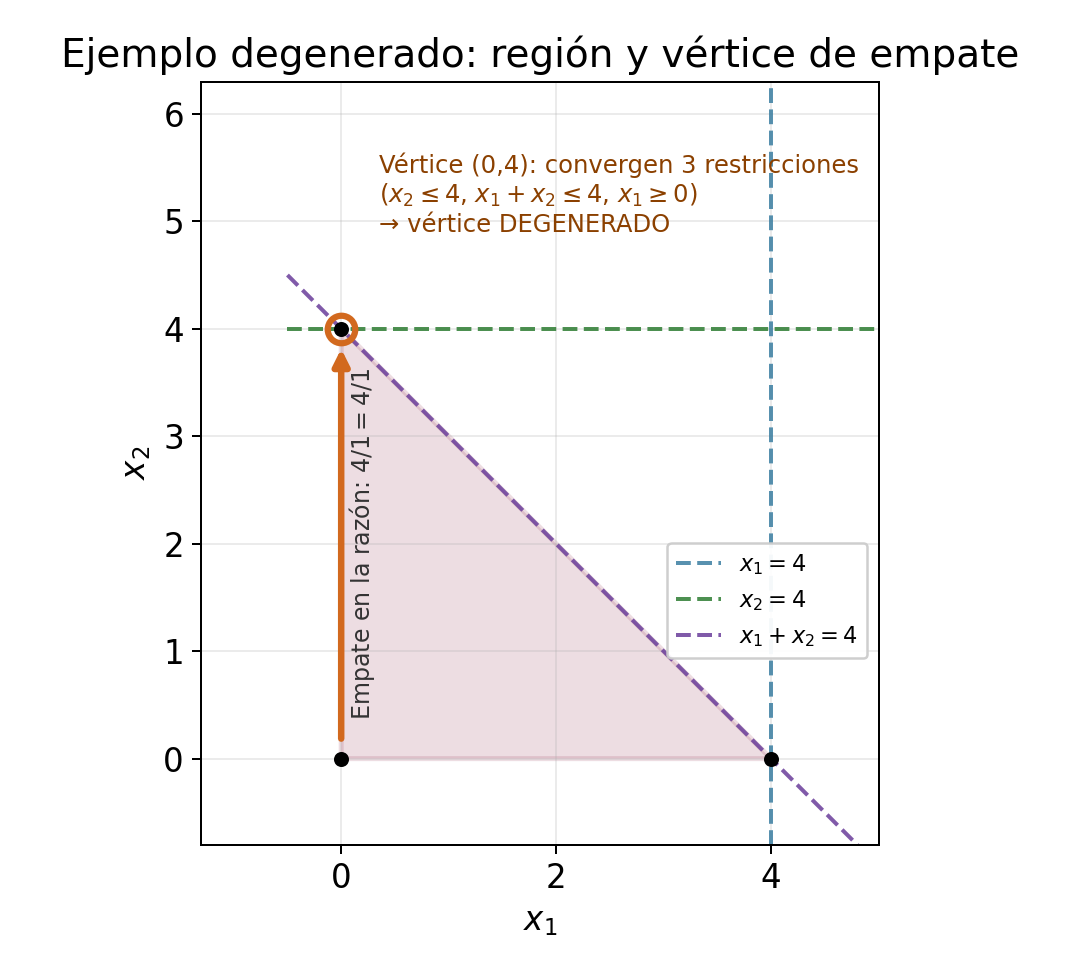
\includegraphics[width=0.46\textwidth]{figs/fig02_region_degenerada.png}

\vspace{-0.05cm}
{\footnotesize En $(0,4)$ convergen simultáneamente $x_2\leq4$ y $x_1+x_2\leq4$ (además de $x_1\geq0$): tres restricciones para un vértice en 2D --- ahí está la degeneración, visible geométricamente antes de tocar el álgebra.}
\end{frame}

\begin{frame}{Resolviendo el empate: regla de Bland}
\begin{alertblock}{Regla de Bland (anticiclado)}
Entre las filas empatadas en la razón mínima, \textbf{sale la variable de menor índice}. (Regla análoga para elegir la variable \textbf{entrante} cuando hay empate de coeficientes en $z$: también el menor índice.)
\end{alertblock}

Con orden $(x_1,x_2,s_1,s_2,s_3)$: $s_2$ tiene índice menor que $s_3$ $\to$ \textbf{sale $s_2$}.

Tras pivotear: nueva SBF $x_1=0,\ x_2=4,\ s_1=4,\ s_2=0,\ s_3=0,\ z=12$.
\par\medskip
\begin{block}{Ya es degenerada}
$s_3=0$ aunque $s_3$ sigue siendo, formalmente, \textbf{variable básica} de esta solución (solo que con valor cero). Es exactamente el vértice $(0,4)$ de la figura, donde tres restricciones coinciden.
\end{block}
\end{frame}

\begin{frame}{El pivote degenerado en acción}
Fila $z$ tras el primer pivote: $z=12+2x_1-3s_2$. Coeficiente de $x_1$ es $+2>0$: \textbf{no es óptimo todavía}. Entra $x_1$.

Razón mínima:
\[
s_1:\ \frac{4}{1}=4 \qquad\qquad s_3:\ \frac{0}{1}=0
\]
\par\medskip
\begin{alertblock}{Aquí está el pivote degenerado}
La razón mínima es $\mathbf{0}$ (fila $s_3$, que ya valía 0). Al pivotear, \textbf{la base cambia} ($s_3$ sale, $x_1$ entra) pero como el paso permitido es 0, \textbf{$z$ no mejora en esta iteración}: sigue en $12$.
\end{alertblock}

Tras este pivote: $x_1=0,\ x_2=4,\ s_1=4$, base $\{s_1,x_2,x_1\}$, $z=12$. La fila $z$ resultante ya no tiene coeficientes positivos: \textbf{óptimo}, $z^\ast=12$ en $(x_1,x_2)=(0,4)$.
\end{frame}

\begin{frame}{¿Por qué esto es peligroso en general?}
\small En este ejemplo pequeño, el pivote degenerado ocurrió \textbf{una sola vez} y el algoritmo terminó normalmente. El riesgo real: en problemas más grandes, \textbf{varios pivotes degenerados consecutivos} pueden revisitar la misma base (o un ciclo de bases) sin que $z$ mejore nunca $\to$ el algoritmo \textbf{no converge}.
\par\normalsize\medskip
\begin{block}{Estrategias anticiclado}
\small
\begin{itemize}
\item \textbf{Regla de Bland} (la que usamos): garantiza teóricamente que el Simplex \emph{nunca} cicla, a cambio de converger a veces más lento que con la regla ``coeficiente más negativo''.
\item \textbf{Perturbación lexicográfica}: perturbar los $b_i$ con cantidades infinitesimalmente distintas ($b_i+\epsilon^i$) para que los empates en la razón mínima ``nunca'' ocurran exactamente --- se rompen en el límite $\epsilon\to0$.
\item En la práctica, los solvers modernos (p.ej. \texttt{HiGHS}, usado por \texttt{scipy}) combinan reglas de pivoteo más sofisticadas con salvaguardas anticiclado --- rara vez se activa Bland ``puro'', pero está ahí como red de seguridad teórica.
\end{itemize}
\normalsize
\end{block}
\end{frame}

\begin{frame}{Síntesis: cómo reconocer y manejar la degeneración}
\begin{center}
\renewcommand{\arraystretch}{1.35}
\begin{tabular}{@{}p{4.6cm}p{7.6cm}@{}}
\toprule
\textbf{Señal} & \textbf{Qué significa / qué hacer}\\
\midrule
Empate en la razón mínima & Más de una fila propone el mismo límite $\to$ aplicar regla de Bland (o cualquier regla de desempate consistente) para decidir cuál sale.\\
Una variable básica en $0$ & La SBF actual es degenerada: geométricamente, un vértice ``sobredeterminado''.\\
Razón mínima $=0$ en una iteración & Pivote degenerado: la base cambia pero $z$ no mejora en ese paso.\\
Muchos pivotes degenerados seguidos & Riesgo (raro pero real) de ciclado; Bland lo previene en teoría.\\
\bottomrule
\end{tabular}
\end{center}
\end{frame}

% ================= SECCION 7 =================
\section{Verificación computacional y síntesis}

\begin{frame}[fragile]{Verificación con \texttt{scipy.optimize.linprog}}
Antes de confiar en cualquier resultado a mano, lo contrastamos con un solver profesional:

\begin{lstlisting}[language=Python]
from scipy.optimize import linprog
res = linprog(
    c=[-3, -5, 0, 0, 0],          # minimiza -z  (linprog minimiza)
    A_eq=[[1,0,1,0,0],
          [0,2,0,1,0],
          [3,2,0,0,1]],
    b_eq=[4, 12, 18],
    bounds=[(0, None)] * 5,
    method="highs",
)
print(res.x, -res.fun)   # -> [2. 6. 2. 0. 0.]  36.0
\end{lstlisting}

Coincide exactamente con lo obtenido a mano y con el tableau: $x_1^\ast=2,\ x_2^\ast=6,\ z^\ast=36$. El mismo patrón se usó para verificar el ejemplo degenerado (también coincide: $z^\ast=12$ en $(0,4)$).
\end{frame}

\begin{frame}{Mapa conceptual del método Simplex}
\begin{center}
\resizebox{!}{0.82\textheight}{%
\begin{tikzpicture}[
  node distance=0.4cm and 0.9cm,
  box/.style={draw, rounded corners, align=center, fill=basecolor!12, minimum width=3.4cm, minimum height=0.9cm, font=\small},
  decision/.style={draw, diamond, align=center, fill=entra!12, minimum width=2.9cm, minimum height=0.9cm, font=\small, aspect=2.2},
  arr/.style={-Stealth, thick}
]
\node[box] (init) {Forma estándar\\+ base inicial (holguras)};
\node[decision, below=of init] (opt) {¿Fila $z$ sin\\coef. positivos?};
\node[box, right=1.6cm of opt] (fin) {ÓPTIMO\\leer $b_i$ de la base};
\node[box, below=of opt] (entra) {Elegir variable\\entrante (Dantzig / Bland)};
\node[decision, below=of entra] (unb) {¿Sin razón\\positiva alguna?};
\node[box, right=1.6cm of unb] (nb) {NO ACOTADO\\$z\to\infty$};
\node[box, below=of unb] (sale) {Razón mínima $\to$\\variable saliente\\(Bland si hay empate)};
\node[box, below=of sale] (piv) {Pivotear:\\normalizar + eliminar\\(Gauss-Jordan)};

\draw[arr] (init) -- (opt);
\draw[arr] (opt) -- node[above, font=\scriptsize]{sí} (fin);
\draw[arr] (opt) -- node[left, font=\scriptsize]{no} (entra);
\draw[arr] (entra) -- (unb);
\draw[arr] (unb) -- node[above, font=\scriptsize]{sí} (nb);
\draw[arr] (unb) -- node[left, font=\scriptsize]{no} (sale);
\draw[arr] (sale) -- (piv);
\draw[arr] (piv.west) -- ++(-2.3,0) |- (opt.west);
\end{tikzpicture}%
}
\end{center}
\end{frame}

\begin{frame}{Lo que ya sabemos hacer}
\begin{itemize}
\item Convertir un problema de PL a forma estándar (holguras).
\item Elegir una base inicial factible y reconocer que el sistema ``ya viene diagonalizado'' para las holguras.
\item Aplicar el criterio de optimalidad, elegir variable entrante, aplicar la razón mínima, y \textbf{diagonalizar a mano} (Gauss-Jordan) para obtener la siguiente SBF.
\item Reconocer que el \textbf{tableau} es la misma álgebra, solo con notación compacta.
\item Detectar y manejar \textbf{empates} en la razón mínima (degeneración) con la regla de Bland, y entender por qué existe el riesgo (remoto) de ciclado.
\item Verificar cualquier resultado con \texttt{scipy.optimize.linprog}.
\end{itemize}
\end{frame}

\begin{frame}{Lo que falta (próxima clase / roadmap)}
\begin{itemize}
\item \textbf{Restricciones $\geq$ o $=$}: no hay una base inicial ``regalada'' de holguras $\to$ método de \textbf{Big M} o método de \textbf{dos fases} (variables artificiales).
\item \textbf{Dualidad}: todo problema de PL tiene un problema ``dual'' asociado; sus soluciones se relacionan con los precios sombra ($z$ de la fila, columnas de holgura) que ya aparecieron en nuestro tableau final.
\item \textbf{Análisis de sensibilidad}: qué tan sensible es $z^\ast$ a cambios en $b_i$ o $c_j$ --- se lee directamente de la fila $z$ y de las columnas de holgura del tableau óptimo.
\item Esto conecta con el roadmap general del curso (Clase 3): tras Newton/cuasi-Newton, PL es la puerta de entrada a la programación no lineal con restricciones (SQP, barreras).
\end{itemize}
\end{frame}

\begin{frame}{Ejercicios propuestos}
\small
\begin{enumerate}
\setlength{\itemsep}{2pt}
\item Resuelva a mano (sistema de ecuaciones, sin tableau) el problema $\max z=5x_1+4x_2$ s.a. $6x_1+4x_2\leq24,\ x_1+2x_2\leq6,\ x_1,x_2\geq0$. Verifique con \texttt{linprog}.
\item Repita el ejercicio anterior usando el formato tableau y confirme que llega a la misma secuencia de bases.
\item Modifique el ejemplo principal cambiando $c_2$ de $5$ a $4.5$: ¿aparece un empate en la fila $z$ al terminar? Interprete qué significa (óptimos múltiples).
\item Construya un ejemplo de 2 variables con un vértice degenerado distinto al de la clase (¿qué debe pasar con 3 rectas para que se crucen en un punto?).
\item Investigue el ejemplo de ciclado de Beale (1955): ¿cuántas variables y restricciones tiene? ¿cuántas iteraciones cicla con la regla de Dantzig antes de repetirse?
\item Para $\max z=x_1-x_2$ s.a. $x_1-x_2\leq1,\ x_1,x_2\geq0$ (no acotado), muestre en qué paso se detecta la ausencia de cota y explique el significado geométrico.
\end{enumerate}
\end{frame}

\begin{frame}{Referencias}
\small
\begin{itemize}
\setlength{\itemsep}{1pt}
\item Dantzig, G. B. (1963). \emph{Linear Programming and Extensions}. Princeton University Press.
\item Bertsimas, D., \& Tsitsiklis, J. N. (1997). \emph{Introduction to Linear Optimization}. Athena Scientific.
\item Hillier, F. S., \& Lieberman, G. J. (2021). \emph{Introduction to Operations Research} (11th ed.). McGraw-Hill. (Origen del ejemplo Wyndor Glass Co.)
\item Vanderbei, R. J. (2020). \emph{Linear Programming: Foundations and Extensions} (5th ed.). Springer.
\item Chvátal, V. (1983). \emph{Linear Programming}. W. H. Freeman.
\item Bland, R. G. (1977). ``New finite pivoting rules for the simplex method''. \emph{Mathematics of Operations Research}, 2(2), 103--107.
\item Beale, E. M. L. (1955). ``Cycling in the dual simplex algorithm''. \emph{Naval Research Logistics Quarterly}, 2(4), 269--275.
\item Nocedal, J., \& Wright, S. J. (2006). \emph{Numerical Optimization} (2nd ed.), Cap. 13. Springer.
\end{itemize}
\end{frame}

\begin{frame}{}
\centering
{\Large\textbf{Gracias}}

\vspace{0.4cm}
\normalsize Preguntas y discusión
\end{frame}

\end{document}
